\chapter{Maximum flows}\label{ch:3}

\section{The \maxflow{}}
An important problem in many applications is to find out the maximum amount of flow that can simultaneously be transferred over a network between two points. % from $s$ to $t$. 
Depending on the context, flow can mean different things, e.g the amount of water in a water pipe system in your city or the bandwidth of a computer network. We call such a network a \textit{flow network}:

\begin{definition}[flow network]
A \textit{flow network} $N$ is a 4-tuple $N=(G,c,s,t)$ consisting of a \textit{digraph} $G$, a positive real-valued capacity function $c: E \rightarrow \mathbb{R}_+ , \forall e \in E : c(e) \geq 0$ defined on all edges of the graph and two designated vertices, the \textit{source} $s \in V$ and the \textit{sink} (or target) $t \in V$ \cite{ahuja1993network}[1.2].
\end{definition}


%However, the links in the network on paths from $s$ to $t$ can only handle flow up to their maximum capacity $c$. One now seeks an assignment of flow values $f$ to edges $e$ that fulfills all the capacity constraints of the edges and the flow conservation property on all the inner nodes, meaning we don't want leaks in our pipe system.
However, the individual links in the network can only handle flow up to their maximum capacity, e.g. they are limited by the diameter of the water pipe. Additionally, the total flow must be preserved at the intermediate joints, e.g. we don't want leaks in our pipe system. This is called a \textit{feasible flow}:% Given such a network, an obvious problem is to find out the maximum amount of flow that can simultaneously be transfered over the network, 


\begin{definition}[feasible flow]
A \textit{feasible flow} $f$ from $s$ to $t$ is a mapping $f : E \rightarrow \mathbb{R}$ satisfying two constraints: The \Eqref{eq:cap} ensures that the flow over an edge is always positive and not exceeding the edge's maximum capacity, while the \Eqref{eq:conserv} assures that the total flow into a vertex $v \notin {s,t}$ equals the total flow out of $v$:
\begin{align}
0 \leq f(e) \leq c(e) & \forall e \in E \eqname*[eq:cap]{capacity constraint} \\
\sum_{e \in \Ein{v}} f(e) = \sum_{e \in \Eout{v}} f(e) & \forall v \in V \setminus \{s,t\} \eqname*[eq:conserv]{flow conservation} \\ \nonumber
\end{align}
\end{definition}

There might be many feasible flows (e.g the zero flow $f = 0 \, \forall e \in E$), but we are especially interested in transferring as much as possible across the network, the \textit{maximum flow}:
\begin{definition}[maximum flow and flow value]
A \textit{maximum flow} $\max \abs{f}$ is a \textit{feasible flow} that maximizes the \textit{flow value} $\abs{f}$, the amount of flow which flows from $s$ to $t$. This is the net flow into the sink $t$ or out of the source $s$:
\begin{align}
\abs{f} = \sum_{e \in \Ein{t}} f(e) = \sum_{e \in \Eout{s}} f(e) \eqname*[eq:flowval]{flow value} \\ \nonumber
\end{align}
\end{definition}


An important concept in the context of flow algorithms is the residual network capturing possible change to $f$, defined by the residual capacities $c'$ and the \textit{residual graph} $G'$:
\begin{definition}[residual graph]
For a flow $f$ in $G=(V,E)$, we can construct the \textit{residual graph} $G' = (V,E')$ by copying all the vertices $v \in V$ from $G$ and for each $e \in E$ adding one or two edges $e'$ to $E'$ with \textit{residual capacity} $c'$ under the following rules \refFigure{fig:residual}:
\begin{description}
\item[forward edge] if $f(e) < c(e)$ for an edge $e=(a,b) \in E$, then add the forward edge $e' = (a,b)$ with residual capacity $c'(e') = c(e) - f(e)$ to $E'$.
\item[backward edge] if $f(e) > 0$ for an edge $e=(a,b) \in E$, then add the backward edge $e' = (b,a)$ with residual capacity $c'(e') = f(e)$ to $E'$.
\end{description}
\end{definition}

\begin{figure}
\centering
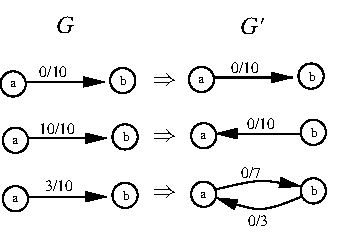
\includegraphics[]{fig/residual}
\caption{Construction of the residual graph $G'$ \cite{mayer2013prakt}.}
\label{fig:residual}
\end{figure}

\clearpage
\section{The \pushRelabel{}}
An early way to compute a maximum flow on a directed graph was called the augmenting path method by Ford-Fulkerson \cite{ford1956maximal}.\footnote{explained in textbooks \cite[sec. 6.4]{ahuja1993network}, \cite[sec. 26.2, p.724]{cormen2009introduction}, \cite[sec. 6.1]{jungnickel2013graphs}} A path with available capacity is an augmenting path, an s-t path in the residual graph. As long as such paths exist, one can increase the flow globally on these paths. If the method terminates, it computes a maximum flow. It is called a method and not an algorithm because the way to find augmenting paths in the residual graph is not fully specified. Furthermore, there is no guarantee on termination and runtime. About 15 years later, two algorithms based on the augmenting path method were developed. They ensure a polynomial time bound by augmenting flow along the shortest path first. The algorithm of Edmonds-Karp \cite{edmonds1972theoretical}\footnote{explained in textbooks \cite[sec. 26.2, p. 727]{cormen2009introduction}, \cite[sec. 6.2]{jungnickel2013graphs}} ensures a runtime of $O(|V|\cdot|E|^2)$ while the one of Dinic \cite{dinic1970algorithm}\footnote{explained in textbooks \cite[sec. 7.4]{ahuja1993network}, \cite[sec. 26.2]{cormen2009introduction}, \cite[sec. 6.4]{jungnickel2013graphs}} improves on that with a runtime of $O(|V|^2\cdot|E|)$. This class of algorithms based on the Ford-Fulkerson method of augmenting paths has been visualized in a previous interdisciplinary project \cite{fischer2016idp}.

Still about another 15 years later, an alternative and more efficient method which uses local operations based on the concept of a preflow and a height function was published: The push-relabel algorithm of Goldberg-Tarjan \cite{goldberg1988new}. In contrast to the previous, less efficient algorithms based on augmenting paths, it changes the flow locally and only needs to construct the residual graph locally. 

\subsection{Excess and height}
The increased efficiency comes at the cost of not maintaining a \textit{feasible flow} during algorithm execution. Instead, a \textit{preflow} is maintained:
\begin{definition}[excess and preflow]
	The \textit{preflow} $\tilde f$ is a generalization of the flow $f$. The \Eqref{eq:cap} of the edges is still maintained, but the \Eqref{eq:conserv} at the vertices is not: The equality sign $=$ is replaced with $\geq$: $\sum_{e \in \Ein{v}} f(e) \geq \sum_{e \in \Eout{v}} f(e) \forall v \in V \setminus \{s\}$.
%This means that more flow can enter an inner node than leaving it, e.g. we allow leaks in our pipe system.
One allows flow \textit{excess}, that is, some vertices can have more incoming than outgoing flow at the intermediate stages of the algorithm \cite{goldberg2014efficient}.  The excess flow at a node $v$ due to the preflow is non-negative for all nodes except for the start node and defined as:
	\begin{align}
		e(v) = \sum_{e \in \Ein{v}} f(e) - \sum_{e \in \Eout{v}} f(e) \geq 0 \quad \forall v \in V \setminus \{s\} \eqname*[eq:excess]{excess} \\ \nonumber
	\end{align}
\end{definition}

\begin{definition}[active node]
As long as a vertex has positive (non-null) excess, it is called an \textit{active node}.
\end{definition}


\begin{remark}
An s-t preflow without active nodes is an s-t flow \cite{matuschke2016network}.	
\end{remark}

Intuitively, we should try to push the excess at a node towards the sink, but what does that mean? Another important concept in the push-relabel algorithm is the height function, which is an approximation of a node's distance to the sink. The local \textit{push} operations try to move \textit{excess} at inner nodes 'downwards' towards the sink. If the current node is at a local minimum and still has excess, we \textit{relabel} the node by increasing its \textit{height} so that subsequent push operations can remove the excess.
\begin{definition}[height, valid labeling]
A \textit{height} function\footnote{also called distance labeling or level function} $h(v) \geq 0 \quad \forall v \in V$ is defined for all vertices of the graph. It is a \textit{valid labeling} of the nodes if it satisfies 
\begin{align}
h(t)=0, h(s)=|V| \quad \text{and} \quad h(v)\leq h(w)+1 \, \forall e'=(v,w) \in E' \eqname*[eq:height]{height} \\ \nonumber	
\end{align}
\end{definition}

\begin{definition}[eligible edge] %or valid with respect to the current height function, 
An edge $e'=(v,w) \in E'$ of the residual graph $G'$ is \textit{eligible} if $h(v)=h(w)+1$, meaning that the current node is one level above the one to where we wish to push excess to.
\end{definition}

\subsection{Termination and runtime}
The important property of the push-relabel algorithm is that when the algorithm terminates, the computed preflow is actually a flow. \textit{This is because there can be no augmenting path from s to t in the residual graph since any such path must contain a steep edge (since s is on level $|V|$, $t$ is on level $0$)} \cite{mehlhorn2000maximum}.

The proof of the runtime involves counting the number of possible saturating and nonsaturating push operations as well as relabel operations. Depending on the way the vertices are selected we get different runtimes, proof sketches in \cite{mehlhorn2000maximum,williamson2007network,matuschke2016network}:
\begin{itemize}
	\item Generic (arbitrary selection rule) with runtime $O(|V|^2 \cdot |E|)$ explained and proved in \cite[sec. 7.6]{ahuja1993network}, \cite[sec. 26.4]{cormen2009introduction}, \cite[alg. 6.6.1]{jungnickel2013graphs}. 
	\item Relabel-To-Front (FIFO selection rule) with runtime $O(|V|^3)$ explained and proved in \cite[sec. 7.7]{ahuja1993network},\cite[sec. 26.5]{cormen2009introduction}, \cite[alg. 6.6.14]{jungnickel2013graphs}.
	\item Highest label selection rule with runtime $O(|V|^2\sqrt{|E|})$ explained and proved in \cite[sec. 7.8]{ahuja1993network} \cite[alg. 6.6.16]{jungnickel2013graphs}.
\end{itemize}

We implemented the Relabel-To-Front variant with the first-in-first-out (FIFO) selection rule. In this variant, a node with excess flow stays active either until a non-saturating push or a relabel occurred. 

\clearpage
\subsection{Pseudocode}
\documentclass[a4paper,11pt]{article}

\usepackage[linesnumbered,ruled,vlined]{algorithm2e}
%\newcommand{\setfont}[1]{\mathcal{#1}}
\newcommand{\setfont}[1]{#1}

\begin{document}

\begin{algorithm}[h!]
\caption{Goldberg-Tarjan Push-Relabel algorithm}
\DontPrintSemicolon % Some LaTeX compilers require you to use \dontprintsemicolon instead
\KwIn{directed Graph $G=(V,E)$ with
\begin{itemize}
	\setlength\itemsep{0pt}
	\setlength{\parskip}{0pt}
	\item digraph $G=(V,E)$ with start $s$, sink $t$
	\item $\forall$ edges $e \in E$: (cap) capacity 
\end{itemize}
}
\KwOut{A feasible maximum s-t flow f(e)}\vspace{0.2cm}
(* Initialize the preflow *)\;
\ForAll{$e=(u,w) \in E$}{
	\If{$u==s$}{
		$f(e) \gets c(e)$\;
		\If{$w \neq t$}{$Q$.add(w)}
	}
	\Else{$f(e) \gets 0$}
}
((* Initialize the height function *))\;
$h(s) = |V|$\;
\ForAll{$v \in V$}{
	$h(v) \gets$ number of arcs on directed v-t path\;
}
((* Main Loop *))\;
\While{$\setfont{Q} \neq \emptyset$}{
	$v \gets \setfont{Q}$.pop()\;
	\While{$e(v)>0$ AND $\exists e'=(v,w) \in E' | h(v)==h(w)+1$}{
		(* Push *)\;
		push $\min(e(v),c'(e'))$ flow from v to w\;
		\If{$w \neq s,t$ AND $w \notin \setfont{Q}$}{
			$\setfont{Q}$.add($w$)\;
		}
	}
	\If{$e(v)>0$ AND $\not\exists e'=(v,w) \in E' | h(v)==h(w)+1$}{
		(* Relabel *)\;
		$h(v) \gets 1 + \min(h(w) | e*=(v,w)\in E'$ \;
		$\setfont{Q}$.add($v$) \;
	}
}
\end{algorithm}


\end{document}
The pseudocode is split into blocks each consisting of a few lines to form different states of the algorithm that can be visualized. This basically transforms the algorithm into a finite state machine, which was first observed in another recent interdisciplinary project \cite{feil2016idp}. The different states are: 1. INITPREFLOW (lines 1-5), 2. INITHEIGHT (lines 6-9), 3. MAINLOOP (lines 10-12), 4. ADMISSIBLEPUSH (line 13), 5. PUSH (lines 14-14), 6. ADMISSIBLERELABEL (line 18) and 7. RELABEL (lines 19-21). For the detailed description of these states we refer to our web application.

 
\clearpage
\subsection{Visualization concept}
\textit{The crucial requirement is [...] $h(v) = h(w) + 1$. Thus we are only allowed to push along [eligible] residual edges $e'=(v,w)$ for which $h(v)$ is exactly one unit larger than $h(w)$ [...]. We may visualize this rule by thinking of water cascading down a series of terraces of different height, with the height corresponding to the labels. Obviously, water will flow down, and [the eligible edge] condition has the effect of restricting the layout of the terraces so that the water may flow down only one level in each step} \cite[sec. 6.6]{jungnickel2013graphs}.

In our visualization concept \refFigure{fig:maxflow}, we show how excess flow $e(v)$ is pushed downwards the terraces of different height $h(v)$. The primary visualization layer displays the graph network, the capacity of an edge and its current flow value. The secondary visualizaiton layer allows to arrange the graph nodes in a 2-dimensional chart, where the axis can be chosen to be y/x (the usual graph), height/id (so that no nodes overlap) or height/excess. The algorithm switches between the different axes depending on the current state.\footnote{The axes can also be kept fixed based on a user request from TU Ilmenau \url{https://github.com/adrelino/idp-graph-algorithms/commit/4f145861dfba5f8305a24c0f9cc4263cf2b17dcf}}

\begin{figure}
\centering
\begin{subfigure}[t]{0.45\textwidth}
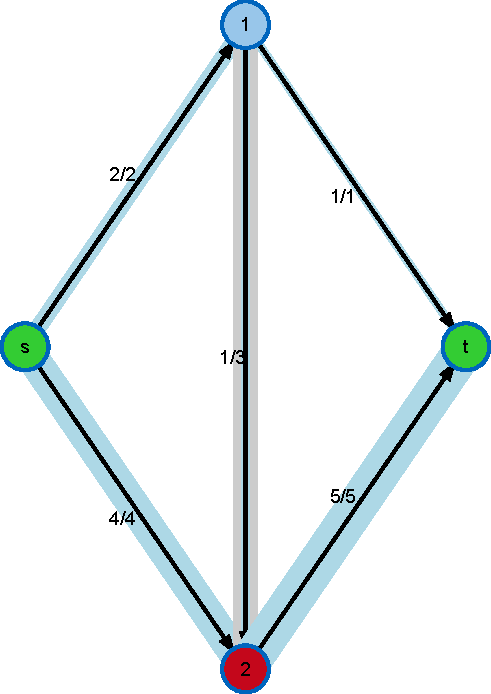
\includegraphics[width=\textwidth]{fig/maxflow-graph-algorithm-graph}
\end{subfigure}
\begin{subfigure}[t]{0.45\textwidth}
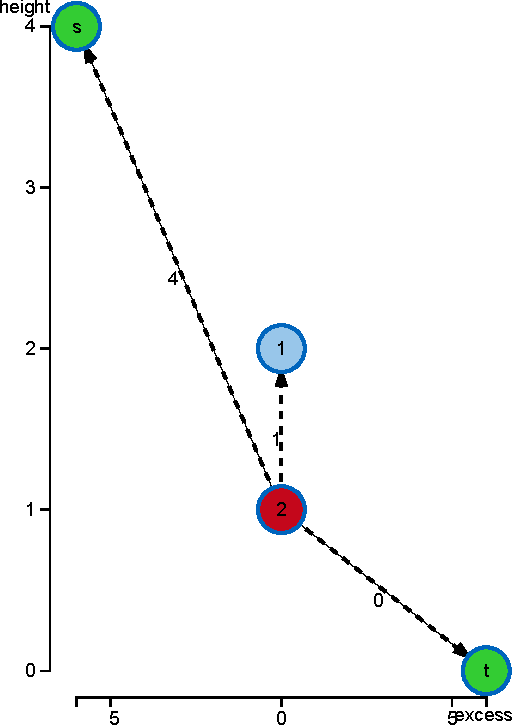
\includegraphics[width=\textwidth]{fig/maxflow-graph-algorithm-height}
\end{subfigure}
\caption{Maxflow concept : The primary visualization layer (left) shows the graph network, with vertices as circles and edges as lines connecting them. Source and target node are coloured in green, the current node in red. The labels of the edges denote the current flow and the maximum capacity in the form flow/cap. The capacity is furthermore drawn as a thick gray line with a width corresponding to its capacity, and the flow is drawn on top of it as a thick blue line. The secondary visualization layer (right) shows the outgoing edges $e'$ of the current node in the residual graph with dashed lines. The nodes are currently arranged according to the height/excess coordinate system axes.}
\label{fig:maxflow}
\end{figure}





